\chapter{Column Databases}

\textbf{Column-oriented systems} (also known as \textbf{column-stores}) are a type of DBMS which store data by column instead of by row. By storing each column separately on disk, queries can read just the attributes they need, without having to read entire rows from disk and then discard what's not needed, which is also useful since physical query plans can be executed one-block-at-a-time (also called \textbf{vectorized execution}) instead of one-tuple-at-a-time, loading multiple records at once for each operator (enough to fill the cache). When compression is considered, columns are easier to compress than rows.
\begin{figure}[h]
    \centering
    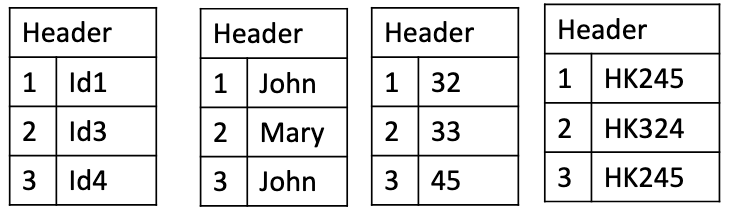
\includegraphics[width=0.5\linewidth]{img/column-store.png}
    \caption{Example of a column-store.}
    \label{fig:column-store}
\end{figure}

They've recently risen in popularity, for reasons related to changes in both applications and technology. Lately, most tasks have become analytical instead of transactional: transactional systems require efficient ways to insert or remove elements, but analytical ones not so much, and instead need efficient ways to read information (which is often a lot). As time goes on, caches become bigger, RAMs become faster, while disk performances change very little. The focus should be on reducing the accesses to disk and instead hold as much information in main memory. Also, the time between transfer time and seek time has widened, so data is often read sequentially. Finally, modern CPUs do instruction pipelining, so ideally function calls should be reduced to a minimum in order to allow the pipeline to execute operations efficiently; they also can execute the same operation in parallel on different parts of the same data structure (SIMD (Single Instruction Multiple Data) parallelism).

The basic trade-off of column-stores can be explained with a simple example. Imagine we have to read a record of 5 attributes. Using row-stores, we'd only have to read the page that contains that record, while with column-stores we'd have to read 5 pages (one per column). If instead we have to read a thousand consecutive tuples of 20 attributes out of which we're interested in 5 of them, then (assuming each page can contain the equivalent of 1000 fields) with a row-store we'd have to read 20 pages, while with a column-store we still have to read only 5 pages. In general, column-stores are advantageous for systems in which reads involve a lot of tuples ($> 1000$) on a restricted set of attributes.

The biggest challenges of column-stores are reconstruction of the tuples, which require a join, and tuple insertion, which takes many I/O operations since all different columns must be updated with the new values (although this is not a big issue in OLAP systems). These problems are exacerbated if the data is compressed.

\section{Storing Columns}

There's two choices in how to store columns. The traditional one is to store them in \textbf{RID order} (as shown in the previous picture): tuples can be reconstructed using a sort-merge-like algorithm, scanning columns in parallel. There's no need to explicitly store RIDs, since they can be inferred as the position of an element within the column.

Another choice is to store them in \textbf{value order}, i.e., they are kept sorted on the value of the tuples. It is extremely convenient for compression via Run Length Encoding, and also permits efficient range searches. This method requires to explicitly store the RIDs. The basic solution is to store them the same way an inverted index does: each value is associated with the list of RIDs which contain it; however, this negates the possibility of compressing the data via RLE, and tuple reconstruction requires an index-nested-loop-like random access algorithm.

Instead of using an inverted index structure, two separate data structures can be used. The first one lists all the values, each followed by the total number of records which have that value (the information is compressed via RLE). The second one is a join index, which specifies the correspondence between the first data structure and some other RID-sorted column.

Overall, using a basic inverted index-like structure is better if we're interested in reconstructing the original tuples; the second method is better if data is going to be kept as separated columns and not reconstructed.

\subsection{C-Store Projections}

The solution used by C-Store (an early column-oriented DBMS) stores each column in a separate file, using a column-specific compression method, and sorting the values according to some attribute in the table. Each column can be stored several times in different sort orders: groups of columns sorted on the same attribute are called \textbf{projections}. If there are sets of columns that are very often requested together, and the query has range searched done on one specific attribute, they can be grouped in a projection and kept sorted on that attribute. The attribute chosen for sorting will also be able to be compressed and allow no-cost GroupBys. If there's other projections sorted on that same attribute, the join done on the other columns is also more efficient (can be done via sort-merge).

Different projections can have overlapping columns. If there's a lot of them, many queries will find their optimal projection, but updates will be slower. To reconstruct the entire table, either a join is done between the different projections using join-indexes, or a big projection is defined to include all columns, capable of answering any query.

\section{Compression}

There have been several research studies that evaluate the performance of different compression algorithms. Some of them can be used on both row and column-stores, while others are specific to column-stores since they allow compression symbols to span across multiple consecutive values.

\paragraph{Run-length Encoding}
RLE compresses runs of the same value in a column to a compact singular representation. Each run is replaced with a triple: (value, starting position, run length). Alternatively, the starting position can be discarded, if we're not interested in that information (for example, if we want to do binary searches on the compressed data).

\paragraph{Bit-Vector Encoding}
Bit-vector encoding compresses columns by representing it with a set of bit vectors, one for each distinct value. Each bit corresponds to a position in the column: if the $i^{th}$ bit is equal to 1, the $i^{th}$ position contains that value, while a 0 means the absence of it. This compression is only useful if the number of distinct values is low.

\paragraph{Dictionary Encoding}
Dictionary encoding is similar to bit-vector encoding, but it maps each value in the column to a different integer, and then represents the column as the sequence of those integers.  It is used for cases in which the datatype of the values requires an high number of bits (strings, usually), so rewriting them as integers will optimize queries. 

\paragraph{Difference Encoding}
When values of a column represent some continuous function, a common way of compressing them is using difference encoding: only the first value is stored, and all the other ones are replaced with the difference with that first one.

\paragraph{Frame of Reference}
Similar to difference encoding, but used when data is stored in multiple pages. Each page is compressed as the first value followed by all differences.

\paragraph{Frequency Partitioning}
With frequency partitioning, similar values are put in the same page; each page is compressed via bit-vector or dictionary encoding.

\subsection{Operating on Compressed Data}

Using compressed data requires some modifications to the query execution engine. RLE encoded data can be operated upon without decompression, as long as there is information about the runs' starting positions. Dictionary encoding also allows range queries for range queries. Bit-vector encoding allows any bit operations on sets.

For any other compression algorithm (or any other operation not included above), tuples must be reconstructed, via either \textbf{early materialization} or \textbf{late materialization}.
\begin{itemize}
    \item Early materialization simply rebuilds the part of the table the query operates on by scanning and joining all the necessary columns, and then using relational algebra.

    \item Late materialization uses column algebra to operate on one column at a time, without needing to reconstruct the table. Each column has two elements: the set of object IDs and the other a string or integer. The operations defined for late materialization are:
    
        $\textbf{select}(\textit{bat}[H,T] AB, \textit{bool} *f(\dots, pi, \dots)) : \textit{bat}[H, \textit{nil}] \\
        = \langle [a, \textit{nil}] | [a,b] \in AB \land f(b, \dots, pi, \dots) \rangle \\
        \textbf{join}(\textit{bat}[T1, T2] AB, bat[T2, T3] CD, \textit{bool} *f(\dots, pi, \dots)) : \textit{bat}[T1,T3] \\
        = \langle [a, d] | [a,b] \in AB \land [c,d] \in CD \land f(b, \dots, pi, \dots) \rangle \\
        \textbf{reconstruct}(\textit{bat}[H,nil] AN, \textit{bat}[H,T] AB) : \textit{bat}[H,T] \\
        = \langle [a,b] | [a,b] \in AB \land [a, nil] \in AN \rangle \\
        \textbf{reverse}(\textit{bat}[H,T] AB) : \textit{bat}[T,H] \\
        = \langle [b,a] | [a,b] \in AB \rangle \\
        \textbf{voidtail}(\textit{bat}[H,T] AB) : bat[H,\textit{nil}] \\
        = \langle [a,\textit{nil}] | [a,b] \in AB \rangle \\
        \textbf{group}(\textit{bat}[\textit{oID}, T] AB) : \textit{bat}[\textit{oID}, \textit{oID}] \\
        = \{[a,o] | o = id_{AB}(b) \land [a,b] \in AB \} \\
        \textbf{sum}(\textit{bat}[\textit{oID}, \textit{int}] AB) : \textit{bat}[\textit{\textit{oID}, \textit{int}} \\
        = [\textit{nil}, \sum\{i | [o,i] \in AB\}]$
\end{itemize}
\begin{figure}[h]
    \centering
    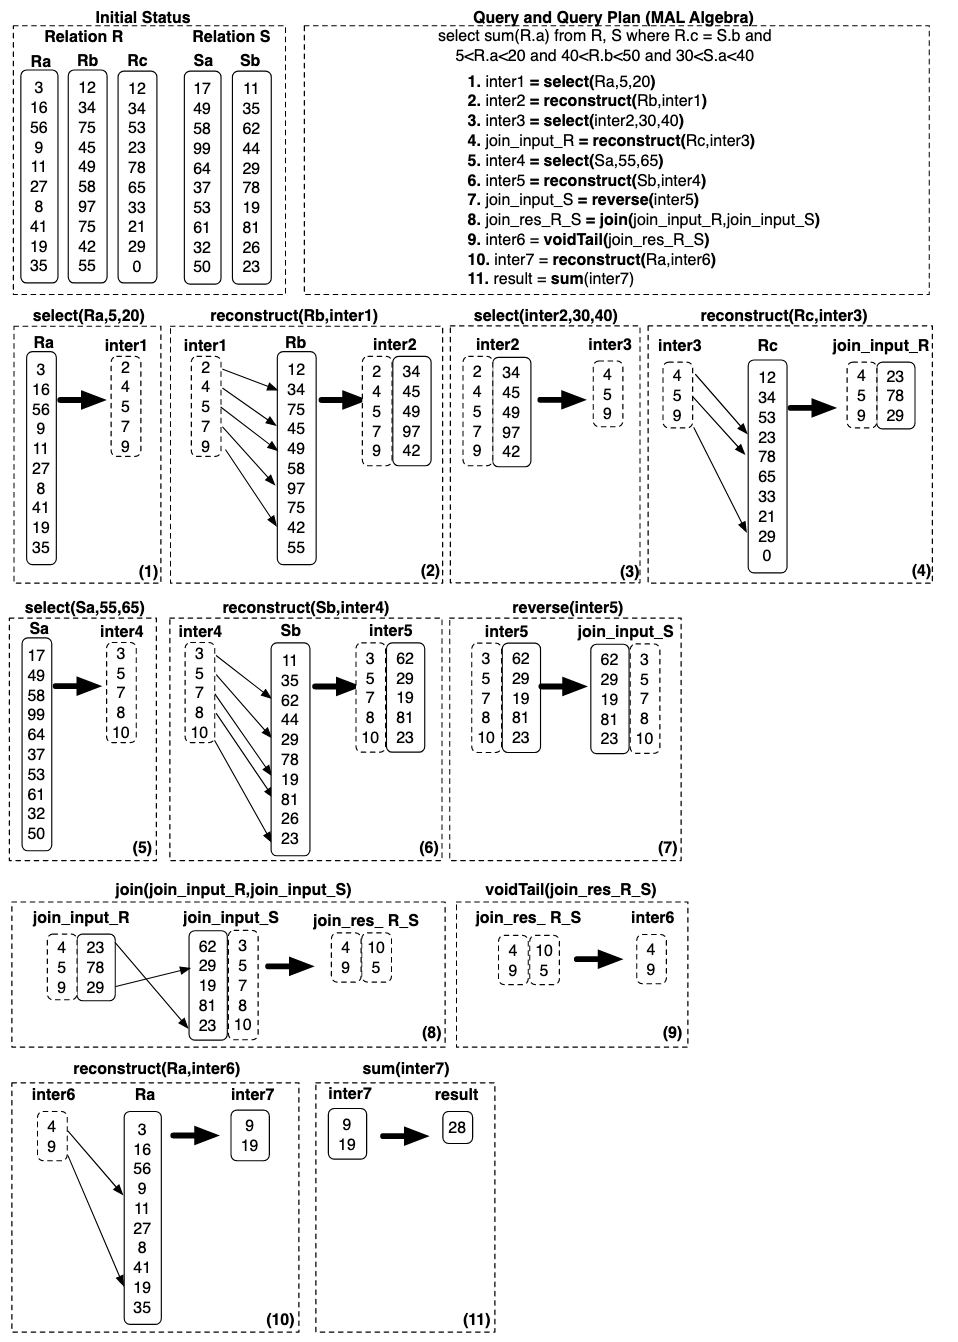
\includegraphics[width=0.75\linewidth]{img/late_materialization.png}
    \caption{Example of late materialization.}
    \label{fig:late-materialization}
\end{figure}

A binary table (``bat'') can be represented in many ways; the result of a select may just be a bitmap, and the result of a reconstruct may be a bitmap in front of the original column.

\section{Column Operations}

\subsection{Column Join}

Since columns avoid using indexes, the algorithms used to join them are HashJoin, SortMerge, or main memory join (since columns are often small enough to fit in main memory). The output of the join is a set of pairs of positions in the input relations for which the predicate succeeded. These pairs can be stored in the form of join indexes, which are often much smaller than the original columns, making subsequent operations faster.

Still, only the positions of the outer relation will be sorted, while the ones in the inner one will not, so accessing those elements will require a lot of jumps in the storage. One solution is to use the \textbf{Jive join}. This algorithm is one-operator-at-a-time, does a single read of the input relations, only blocks where one tuple that is named in the join index is present are read, and returns a result in column form (unsorted). Assume we have two tables, $R$ and $S$, both with their respective record IDs and a set of attributes, out of which only one is the join attribute:
\begin{gather*}
    R(RID, A, B), \ S(SID, BB, C) \\
    \pi_{ABC}(R \bowtie_{B=BB} S) 
\end{gather*}
Assume we also have a join index:
\begin{equation*}
    JI = \pi_{RID, SID} (R \bowtie_{B=BB} S)
\end{equation*}
Also, let $N_{pag}$ be the number of pages in the projected and semijoined $S$ plus the number of pages in the join index, then:
\begin{equation*}
    2*N_{pag} < B*B
\end{equation*}
There's no limit on $R$. To explain how the algorithm works, it is best to use an example. We have two tables:
\begin{figure}[H]
\centering
    \begin{minipage}{0.49\textwidth}
    \centering
        \begin{tabular}{|c|c|}
        \hline
            1 & Johnson \\
        \hline
            2 & Jones \\
        \hline
            3 & Johnson \\
        \hline
            4 & Doe \\
        \hline
            5 & Smith \\
        \hline
        \end{tabular}
    \end{minipage}
    \hfill
    \begin{minipage}{0.49\textwidth}
    \centering
        \begin{tabular}{|c|c|}
        \hline
            1 & Smith \\
        \hline
            2 & Johnson \\
        \hline
            3 & Williams \\
        \hline
            4 & Jones \\
        \hline
        \end{tabular}
    \end{minipage}
\end{figure}
\noindent The join produces the following join index:
\begin{table}[H]
    \centering
    \begin{tabular}{|c||c|}
    \hline
        1 & 2 \\
    \hline
        2 & 4 \\
    \hline
        3 & 2 \\
    \hline
        5 & 1 \\
    \hline
    \end{tabular}
\end{table}
\noindent As it can be seen, the outer relation RIDs are sorted. To sort the inner relation ones, we add an additional column to that list, containing an increasing sequence of integers:
\begin{table}[H]
    \centering
    \begin{tabular}{|c||c|}
    \hline
        2 & 1\\
    \hline
        4 & 2\\
    \hline
        2 & 3\\
    \hline
        1 & 4\\
    \hline
    \end{tabular}
\end{table}
\noindent This output is then sorted by the list of RIDs, causing the newly added column to be out of order:
\begin{table}[H]
    \centering
    \begin{tabular}{|c||c|}
    \hline
        1 & 4\\
    \hline
        2 & 1\\
    \hline
        2 & 3\\
    \hline
        4 & 2\\
    \hline
    \end{tabular}
\end{table}
\noindent The column from the inner table is scanned in order with values at the (now sorted) list of positions extracted and added to the current data structure:
\begin{table}[H]
    \centering
    \begin{tabular}{|c||c|c|}
    \hline
        1 & 4 & Smith \\
    \hline
        2 & 1 & Johnson \\
    \hline
        2 & 3 & Johnson \\
    \hline
        4 & 2 & Jones \\
    \hline
    \end{tabular}
\end{table}
\noindent And finally, the data structure is sorted by the added column, reverting it to the original join order:
\begin{table}[H]
    \centering
    \begin{tabular}{|c||c|c|}
    \hline
        2 & 1 & Johnson \\
    \hline
        4 & 2 & Jones \\
    \hline
        2 & 3 & Johnson \\
    \hline
        1 & 4 & Smith \\
    \hline
    \end{tabular}
\end{table}
\noindent Now, all columns can be iterated through sequentially, at the cost of two sorts of the join output data. The sorting is done by using $2*k$ buffers to create $2*k$ files with the join index and temporary sorted join index.

\subsection{Column GroupBy and Aggregation}

GroupBy is typically hash-based, unless the input is already sorted according to the groupby attributes. Aggregation exploit the column layout very efficiently: they can work on only the relevant column with tight for loops.

\subsection{Column Insert, Update, Delete}

Insertion is very expensive in column-stores, because inserts must update all columns, and if the columns are ordered, the insertion must also respect the ordering. Also, systems such as C-Store use a lot of duplication, increasing the cost even further. The same problems hold for updates and deletes.

A solution is to use differential files, stored in memory, so that all operations can be done all at once. Some database systems (such as C-Store) handle updates by splitting their architecture into a \textbf{read-store} that manages the bulk of data, and a \textbf{write-store} (kept in main memory) that manages updates that have been made recently. The read-store is read-optimized, while the write-store is compact. Every query requests both the read-store and the write-store and merges the two results. This approach requires to explicitly store RIDs.

The write-store can be used to implement SNAPSHOT isolation, where the read-store can be seen as the snapshot of the write-store. It also allows easy implementation of the no-undo/redo algorithm, making sure that the write-store is a sort of redo log that is merged only after commit.

\subsection{Indexing}

A sorted column on an attribute $A$ with a join index can be seen as equivalent to a traditional index on $A$. Similarly, a projection $\{A_1, A_2, \dots, A_n | A_i\}$ is like an index on $A_i$ which allows queries to rapidly access $A_1, \dots, A_n$, using an IndexOnly plan. Creating actual indexes on each column of a relation will not work well: tuple reconstruction will still require joins of the index with the original table, and introduce insert/delete overhead.

Alternatively, we may split the table $R(A,B,C,\dots)$ as a set of separate columns $R_1(IdA, A)$, $R(IdA, B)$, $R(IdA, C)$, $\dots$, where $IdA$ is a small integer, and all the tables are sorted on it. This allows fast joins, but does not allow compression, forces a pipelined execution, and still introduces overhead for insert/delete operations as well as index accessing. Also, lots of joins may confuse the optimizer, ending up with costlier plans.